\chapter{Resultados Obtidos}
\label{cap:ResultadosObtidos}

Como resultado do desenvolvimento do modelo OLAP e dos processos de ETL através dos \emph{scripts} em Python descritos nos capítulos anteriores, após a carga de inicial das informações, foi possível executar a criação do cubo de dados e suas respectivas dimensões dentro do \emph{Microsoft Analysis Services}. 

Nos primeiros testes realizados no cubo de dados, em conjunto com os especialistas de domínio, foi identificado que através da análise da FEB média utilizando como ligante o TCL o resultado agregado apresentava um valor positivo. 

Inicialmente acreditou-se que poderia ter sido algum problema durante o processo de ETL ou alguma regra de negócio que não estava sendo devidamente contemplada. Porém, ao avaliar o \emph{data set} original contendo os dados de experimentos de docagem molecular, viu-se que grande parte dos melhores valores resultantes de FEB para o ligante TCL eram posivitos.

Com isso, os especialistas de domínio definiram que qualquer resultado de FEB que apresentasse valor positivo poderia ser desconsiderado. Neste caso, foi sugerido que tivessem seus valores alterados para zero, conforme descrito na seção \ref{sec:IdentificacaoDeMetricas}. Em função desta definição os \emph{scripts} impactados foram devidamente alterados, sendo necessário realizar uma nova carga de dados e gerar novamente o cubo de dados. 

Enfim, após a segunda carga o valor agregado médio de FEB para o experimento estava sendo apresentado corretamente. A tabela fato foi populada com um total de 6.200 registros, sendo 3.100 deles relacionados aos dados do experimento de docagem executado com o ligante TCL e os outros 3.100 relacionados ao experimento para o ETH. A Figura \ref{fig:TabPivotante} ilusta a tabela pivotante após a carga de dados.

\begin{figure}[h]
        \center
        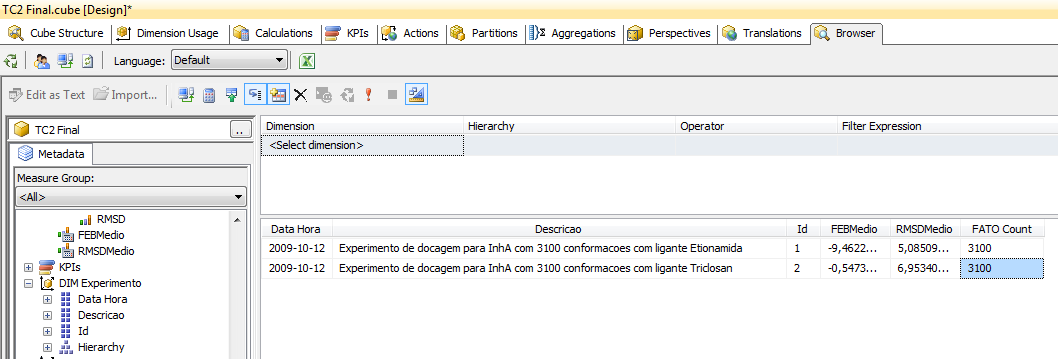
\includegraphics[scale=0.45]{images/TabelaPivotante.PNG}
        \caption{Tabela pivotante do modelo OLAP.}
        \label{fig:TabPivotante}
\end{figure}

Apartir deste momento, foi utilizada a integração da ferramenta Microsoft Excel, servindo como \emph{front-end} para realizar a consulta e análise dos dados presentes no cubo. Como resultado, foi possível navegar entre as dimensões e em suas hierarquias, selecionar os elementos disponíveis e montar os relatórios de dados conforme as necessidades identificadas no início deste projeto. A Figura \ref{fig:excelFull} ilustra o ambiente do Microsoft Excel já integrado.

\begin{figure}[h]
        \center
        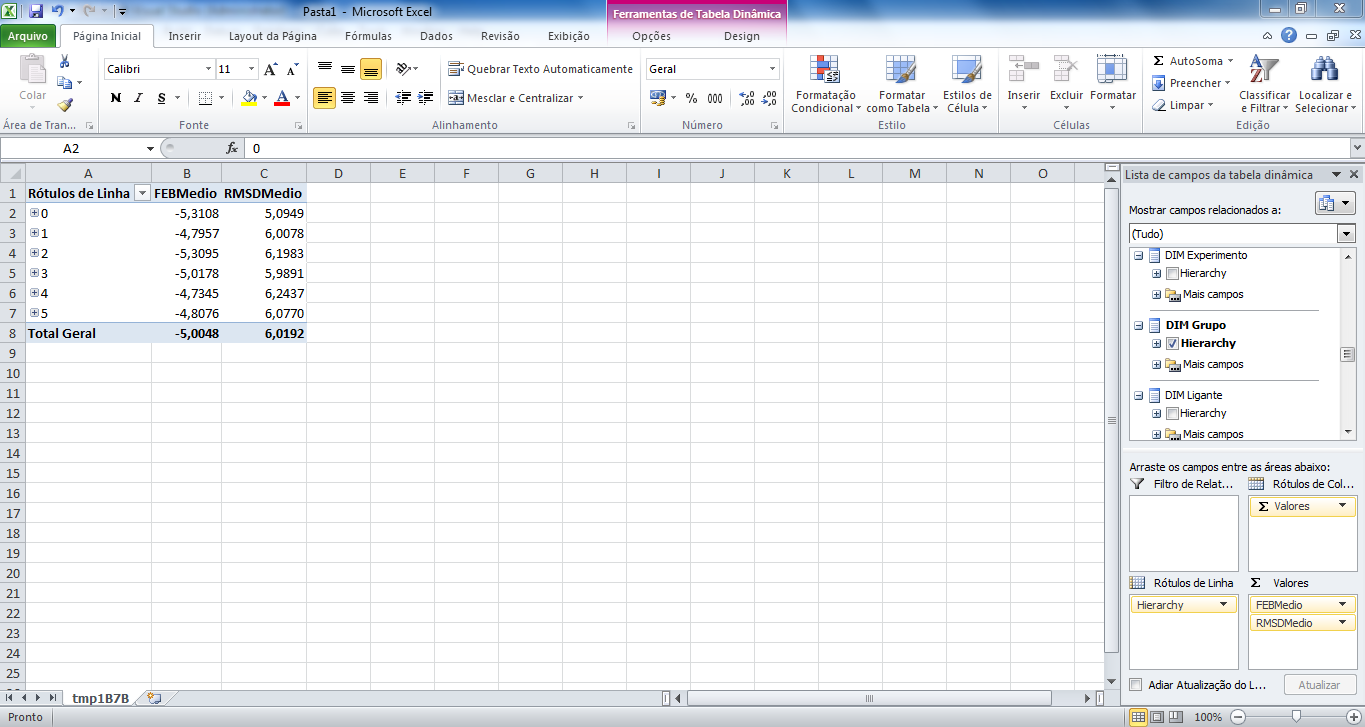
\includegraphics[scale=0.45]{images/ExcelFull.PNG}
        \caption{Ambiente do Microsoft Excel como front-end para análise de dados do cubo}
        \label{fig:excelFull}
\end{figure}

Para responder a primeira questão de negócio, foram selecionados os elementos ``Grupo'' e ``Conformações''. Desta forma é possível visualizar o total de conformações separadas por tipo de agrupamento. A Figura \ref{fig:questao1} ilustra o resultado desta consulta.

\begin{figure}[h]
        \center
        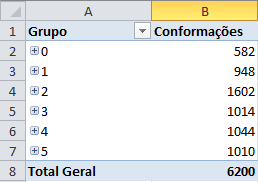
\includegraphics[scale=1]{images/Questao1.PNG}
        \caption{Questão 1 - Visualização das conformações por agrupamento.}
        \label{fig:questao1}
\end{figure}

Para responder a segunda questão de negócio, foram selecionados os elementos ``Grupo'', ``Conformações'', ``FEBMedio'' e ``RMSDMedio''. Para este caso, é possível obter o comportamento das conformações baseado nas métricas de FEB e RMSD, podendo ser agregadas por agrupamento ou não. A Figura \ref{fig:questao2} ilusta o resultado desta consulta.

\begin{figure}[h]
        \center
        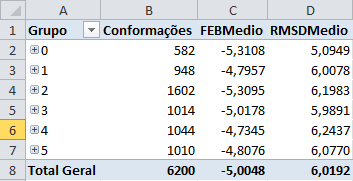
\includegraphics[scale=0.8]{images/Questao2.PNG}
        \caption{Questão 2 - Métricas de FEB e RMSD agregadas por agrupamento}
        \label{fig:questao2}
\end{figure}

Para responder a terceira questão de negócio, foram selecionados os elementos ``Grupo'', ``Ligantes'', e ``Numero Contatos R1'' até ``Numero Contatos R10''. Dessa forma, é possível avaliar as conformações e grupos que possuem o maior número de contatos que os ligantes estabeleceram com os dez resíduos mais relevantes para o experimento. A Figura \ref{fig:questao3} ilustra o resultado desta consulta exibindo apenas sete dos dez principais resíduos.

\begin{figure}[h]
        \center
        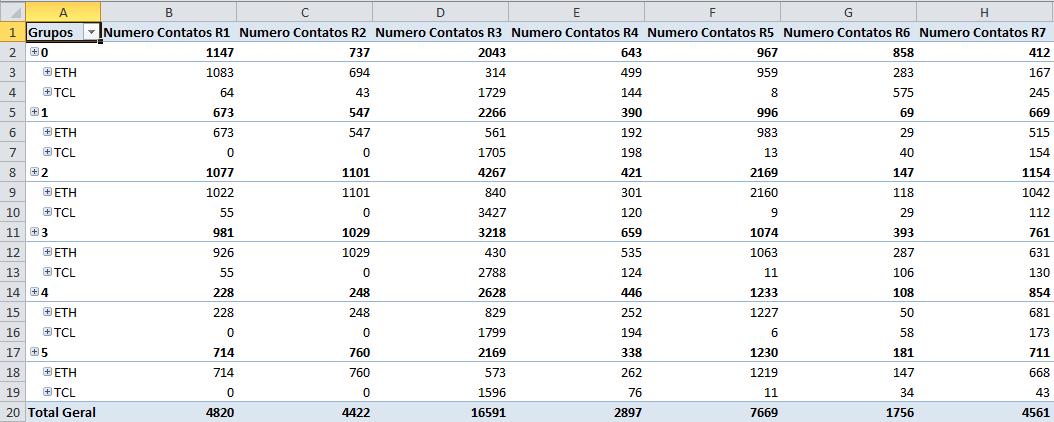
\includegraphics[scale=0.58]{images/Questao3.PNG}
        \caption{Questão 3 - Número de contatos dos principais resíduos agregados por conformações/grupo.}
        \label{fig:questao3}
\end{figure}

Para responder a quarta questão de negócio, foram selecionados os elementos ``Grupo'' e ``Numero Contatos R1'' até ``Numero Contatos R10''. Neste caso, é possível identificar quais são os resíduos mais importantes baseado nas conformações/grupos que os estabeleceram um maior numero de contatos entre os ligantes e os dez resíduos mais relevantes para o experimento. A Figura \ref{fig:questao4} ilustra esta consulta, exibindo apenas para dois agrupamentos. 

\begin{figure}[h]
        \center
        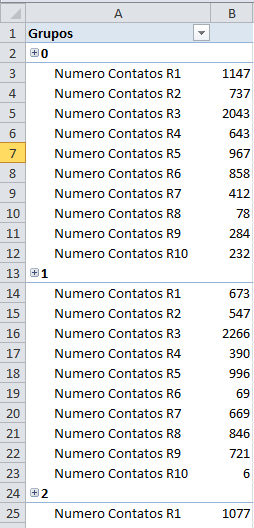
\includegraphics[scale=0.7]{images/Questao4.PNG}
        \caption{Questão 4 - Resíduos mais importantes agregados por conformações/grupo que estabeleceram maior número de ligações.}
        \label{fig:questao4}
\end{figure}

Enfim, para responder a quinta questão de negócio, foram selecionados os elementos ``Grupo'', ``FEBMedio'', ``RMSDMedio'' e ``Experimento''. Com isso, é possível identificar quais agrupamentos possuem melhores valores de FEB e RMSD de acordo com o tipo de experimento realizado. A Figura \ref{fig:questao5} ilustra esta consulta.

\begin{figure}[h]
        \center
        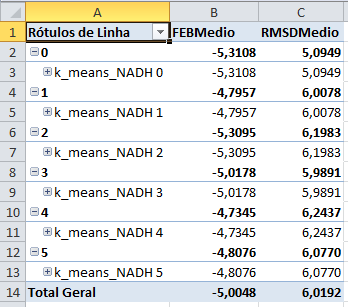
\includegraphics[scale=0.8]{images/Questao5.PNG}
        \caption{Questão 5 - Valores de FEB e RMSD agregados por agrupamento e tipo de experimento.}
        \label{fig:questao5}
\end{figure}

